	 \section{Some applications}
\epigraph{\textit{First law of Physical Mathematics: every cloud has a silver lining.}}{Yuri Manin}
\vspace{10 mm}
\subsection{Calabi-Yau categories}

A natural condition to impose on our triangulated category is to behave just like the derived category of a variety, i.e. to posses some form of Serre duality. This is done in \cite{bon}. In particular, accordingly to our string-theoretic motivations, one can define Calabi-Yau triangulated categories as in \cite{kel}, and try to describe their slicings. \\
Suppose that $\mathscr{D}$ is $k$-linear over some field $k$ (we also assume that $\Sigma$ is $k$-linear). 

\begin{center}
\begin{figure}[h]
\begin{tikzpicture}
\node[opacity=0.7] at (6,0) {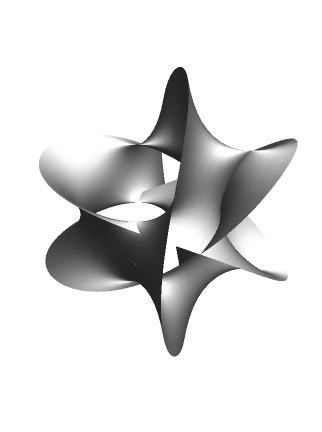
\includegraphics[width=6cm]{Sezione}};  %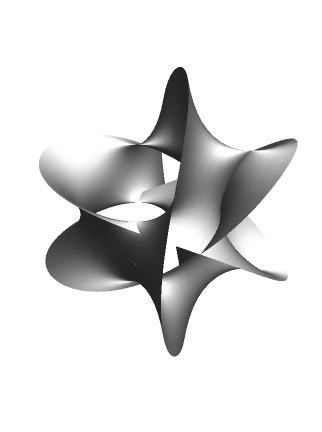
\includegraphics[scale=0.5]{Sezione}
\end{tikzpicture}
\caption{A depiction of a $3$-dimensional real projection of a complex $2$-dimensional section of the Fermat quintic in the $4$-dimensional complex projective space.}
\end{figure}
\end{center}

\begin{defn}
$\mathscr{D}$ is \textbf{Hom-finite} if for each $X,Y \in \mathscr{D}$ the graded $k$-vector space $$\textnormal{Hom}_{\mathscr{D}}^{\bullet}(X,Y)=\bigoplus_{i \in \mathbb{Z}} \textnormal{Hom}_{\mathscr{D}}(X,Y[i])$$ is finite dimensional. 
%If that's the case, we define the \textbf{Euler pairing} $$\chi(X,Y)= \sum_{i \in \mathbb{Z}} (-1)^i \textnormal{dim}_k(\textnormal{Hom}_{\mathscr{D}}(X,Y[i]))$$
\end{defn} 

Suppose moreover that $\mathscr{D}$ is Hom-finite. \\

\begin{defn}
A \textbf{Serre functor} on $\mathscr{D}$ is a $k$-linear autoequivalence $S$ so that there is a natural isomorphism of $k$-linear bifunctors from $\mathscr{D}^{\textnormal{op}} \times \mathscr{D}$ to $\textnormal{Mod}_k$: $$\textnormal{Hom}_{\mathscr{D}}(X,Y) \overset{\varphi_{X,Y}}{\longrightarrow} \textnormal{Hom}_{\mathscr{D}}(Y,S(X))^{\vee}$$
where $*^{\vee}=\textnormal{Hom}_k(*,k)$ denotes the duality functor. \\
If $n \in \mathbb{Z}$, we say that $\mathscr{D}$ is $n$-\textbf{Calabi-Yau} over $k$ if $\Sigma^n$ is a Serre functor on $\mathscr{D}$. We'll often refer to the above isomorphism as \textbf{Serre duality}.
\end{defn} 

First of all, observe that if $S$ is a Serre functor on $\mathscr{D}$, by bifunctoriality we have for each $X,Y \in \mathscr{D}$ a commutative diagram:
\begin{center}
\begin{tikzcd}[ampersand replacement=\&]
 \textnormal{Hom}_{\mathscr{D}}(X,Y)  \arrow{r}{\varphi_{X,Y}} \arrow{d}{S} \& \textnormal{Hom}_{\mathscr{D}}(Y,S(X))^{\vee}  \\ 
\textnormal{Hom}_{\mathscr{D}}(S(X),S(Y)) \arrow{r}{\varphi_{S(X),S(Y)}} \& \textnormal{Hom}_{\mathscr{D}}(S(Y),S^2(X))^{\vee} \arrow{u}{S^{\vee}}
\end{tikzcd}
\end{center}
which will legitimate us to write, as usual, equalities instead of isomorphisms. \\

\begin{exmp}
Let $A$ be a finite-dimensional algebra over $k$. Following \cite{kel}, the bounded derived category of finite dimensional $A$-modules $\mathscr{D}^b(\textnormal{Mod}_A^{\textnormal{fd}})$ has a Serre functor if and only if $A$ is of finite global dimension. In this case, the Serre functor is diven by the Nakayama functor $$\mathscr{L} A^{\vee} \otimes_A *$$ 
\end{exmp}

\begin{prop}
$\mathscr{D}$ admits a Serre functor if and only if for each $X \in \mathscr{D}$ the functor $\textnormal{Hom}_{\mathscr{D}}(X,*)^{\vee}$ from $\mathscr{D}^{\textnormal{op}}$ to $\textnormal{Mod}_k$ is representable. Moreover, the Serre functor, if it exists, is unique up to natural isomorphism of $k$-linear functors.
\end{prop}

\begin{proof}
Clearly, if $S$ if a Serre functor on $\mathscr{D}$, $S(X)$ represents $\textnormal{Hom}_{\mathscr{D}}(X,*)^{\vee}$. Conversely, for each $X \in \mathscr{D}$, choose a representative $S(X)$ for the functor $\textnormal{Hom}_{\mathscr{D}}(X,*)^{\vee}$ and a natural isomorphism of $k$-linear functors $$\textnormal{Hom}_{\mathscr{D}}(*,S(X)) \overset{\varphi_X}{\longrightarrow} \textnormal{Hom}_{\mathscr{D}}(X,*)^{\vee}$$
and this is the data that gives the desired Serre functor. \\
For the second part of the claim, if $S$ and $S'$ are Serre functors, then for each $X \in \mathscr{D}$, $S(X)$ and $S'(X)$ both represent the functor $\textnormal{Hom}_{\mathscr{D}}(X,*)^{\vee}$ and thus $S=S'$ by the Yoneda lemma. 
\end{proof}

\begin{prop}
Let $S$ be a Serre functor on $\mathscr{D}$. Then: 
\begin{enumerate}
\item $S$ commutes (up to natural isomorphism) with all the autoequivalences of $\mathscr{D}$
\item $S$ is a triangle functor 
\end{enumerate}   
\end{prop}

\begin{proof}
Pick an autoequivalence $F$ of $\mathscr{D}$. For each $X, Y \in \mathscr{D}$, using Serre duality we get: 
\begin{align*}
\textnormal{Hom}_{\mathscr{D}}(X,F(S(Y))) & =   \textnormal{Hom}_{\mathscr{D}}(F^{-1}(X),S(Y)) \\
 & =  \textnormal{Hom}_{\mathscr{D}}(Y,F^{-1}(X))^{\vee} \\
& = \textnormal{Hom}_{\mathscr{D}}(F(Y),X)^{\vee} \\
& =  \textnormal{Hom}_{\mathscr{D}}(X,S(F(Y)))
\end{align*}
Using the Yoneda lemma we conclude $FS(Y)=SF(Y)$ naturally, as desired. \\
Now we prove \textit{(2)}. First of all, using \textit{(1)}, there is an isomorphism $S \Sigma = \Sigma S$. Pick a distinguished triangle $X \overset{f}{\longrightarrow} Y \overset{g}{\longrightarrow} Z \longrightarrow $ in $\mathscr{D}$. Now, since for each $E \in \mathscr{D}$ $$\textnormal{Hom}_{\mathscr{D}}(E,*)=\textnormal{Hom}_{\mathscr{D}}(*,S(E))^{\vee}$$ 
and $\textnormal{Hom}_{\mathscr{D}}(*,S(E))^{\vee}$ is cohomological, we have that the triangle $S(X) \longrightarrow S(Y) \longrightarrow S(Z) \longrightarrow$ is special. Putting $C=\textnormal{cone}(S(f))$, we get a distinguished triangle $S(X) \longrightarrow S(Y) \longrightarrow C \overset{h}{\longrightarrow}$. By applying the Hom-functors to these two triangles and using Serre duality we get a commutative diagram with exact rows and columns: 
\begin{center}
\scalebox{0.8}{
\begin{tikzcd}[ampersand replacement=\&]
 \cdots \arrow{r} \& \textnormal{Hom}_{\mathscr{D}}(X[1],Y) \arrow{r} \arrow{d} \& \textnormal{Hom}_{\mathscr{D}}(C,S(Y)) \arrow{r} \arrow{d} \&  \textnormal{Hom}_{\mathscr{D}}(Y,Y) \arrow{r} \arrow{d} \& \cdots \\
\cdots \arrow{r} \& \textnormal{Hom}_{\mathscr{D}}(X[1],Z) \arrow{r} \arrow{d} \& \textnormal{Hom}_{\mathscr{D}}(C,S(Z)) \arrow{r}{d} \arrow{d}{\delta} \&  \textnormal{Hom}_{\mathscr{D}}(Y,Z) \arrow{r} \arrow{d} \& \cdots \\
\cdots \arrow{r} \& \textnormal{Hom}_{\mathscr{D}}(X,X) \arrow{r} \& \textnormal{Hom}_{\mathscr{D}}(C,S(X)[1]) \arrow{r} \&  \textnormal{Hom}_{\mathscr{D}}(Y,X[1]) \arrow{r}  \& \cdots \\
\end{tikzcd}
}
\end{center}
By some diagram chasing involving  \hyperref[a]{\textbf{Proposition \ref*{a}}}, we get a morphism $C \overset{a}{\longrightarrow} S(Z)$ so that $d(a)=g$ and $\delta(a)=h$. This means that the following is a morphism of special triangles: 
\begin{center}
\begin{tikzcd}[ampersand replacement=\&]
S(X) \arrow{r} \arrow{d}{1} \& S(Y) \arrow{r} \arrow{d}{1} \& C \arrow{r} \arrow{d}{a} \& S(X)[1] \arrow{d}{1} \\
S(X) \arrow{r}\& S(Y) \arrow{r}  \& S(Z) \arrow{r}  \& S(X)[1]  
\end{tikzcd}
\end{center}
Applying \hyperref[c]{\textbf{Proposition \ref*{c}}} we get $C=S(Z)$, as desired. 
\end{proof}

\begin{exmp}
If $M$ is an $n$-dimensional complex smooth projective variety, then the classical Serre duality in geometry tells us that the twist $* \otimes \omega_M[n]$ (where $\omega_M$ is the canonical bundle) is a Serre functor on $\mathscr{D}^b(\textnormal{Coh}(M))$. If $M$ is moreover a Calabi-Yau variety (i.e. the canonical bundle $\omega_M=\mathcal{O}_M$ is trivial) then we see that $\mathscr{D}^b(\textnormal{Coh}(M))$ is $n$-Calabi-Yau over $\mathbb{C}$, which is the reason of our nomenclature.  
\end{exmp}
%
%Observe that if $A \subseteq \mathscr{D}$ is a full subcategory and $S$ is a Serre functor, then $S(^{\perp}A)=A^{\perp}$. \\
%
%\begin{prop}
%Suppose that $\mathscr{D}$ has a Serre functor $S$ and that $J$ acts trivially on $\mathbb{Z}$. Let $\mathscr{P}$ be a $J$-slicing on $\mathscr{D}$. Then $\mathscr{P}_{\phi}$ is admissible and has a Serre functor for each $\phi \in J$. 
%\end{prop}
%
%\begin{proof}
%Since $\mathscr{P}_{\phi}$ is a t-structure on $\mathscr{P}_{]-\infty, \phi]}$ fixed by translation and the same holds for $\mathscr{P}_{]-\infty, \phi]}$ in $\mathscr{D}$, by ??? we can suppose $J=[2]$. Pick a t-structure $\mathfrak{t}$ on $\mathscr{D}$ fixed by translation and consider the $[2]$-slicing $\mathscr{P}=\{ \mathfrak{t}^{\perp}, \mathfrak{t} \}$. By the above observation, acting by $S$ on $\mathscr{P}$ we obtain a $[2]$-slicing $$S.\mathscr{P}=\{ S(\mathfrak{t}$$
%\end{proof}

Now, observe that we allow 'negative dimension' ($n \le 0$) in the definition of $n$-Calabi-Yau categories. Such categories exist (see \cite{hol}) and provide a counterexample to the existence of bounded t-structures, as shown below. 

\begin{prop}
Suppose that $\mathscr{D}$ is $n$-Calabi-Yau with $n<0$. Then any t-structure on $\mathscr{D}$ is fixed by translation. In particular, $\mathfrak{bts}(\mathscr{D})=\emptyset$. 
\end{prop}

\begin{proof}
Let $\mathfrak{t}$ be a t-structure on $\mathscr{D}$. For each $X \in \heartsuit_{\mathfrak{t}}$, using Serre duality  $$\textnormal{End}_{\mathscr{D}}(X)=\textnormal{Hom}_{\mathscr{D}}(X[-n],X)^{\vee}$$
Since $n<0$, the latter is zero and thus $X=0$. By arbitrariness of $X$, $\heartsuit_{\mathfrak{t}}=0$, as desired. \\
The second claim follows from the fact that if a t-structure is fixed by translation then it has zero heart, and thus can't be bounded. 
\end{proof}

\begin{prop}\label{tta}
Suppose that $\mathscr{D}$ is $n$-Calabi-Yau. Suppose moreover that one of the following conditions holds: 
\begin{enumerate} 
\item $n \le 1$ 
\item the action of $\mathbb{Z}$ on $J$ is trivial 
\end{enumerate}  
Then any $J$-slicing on $\mathscr{D}$ is hereditary. 
\end{prop}

\begin{proof}
Pick $X \in \mathscr{P}_{\phi}$, $Y \in \mathscr{P}_{\psi}$ and suppose $\phi + 1 < \psi$ in $J$. Then using Serre duality we get $$\textnormal{Hom}_{\mathscr{D}}(X,Y)=\textnormal{Hom}_{\mathscr{D}}(Y,X[n])^{\vee}$$
Now, $X[n]$ is semistable of phase $\phi + n $ with respect to $\mathscr{P}$. If condition \textit{(1)} holds, then $\phi + n \le \phi + 1 < \psi$. It condition \textit{(2)} holds, then $\phi + n = \phi < \psi$. In either case, the latter is zero, as desired. 
\end{proof}

\begin{prop}\label{ttb}
Let $M$ be an $n$-dimensional Calabi-Yau variety and suppose that the action of $\mathbb{Z}$ on $J$ is trivial. Then any $J$-slicing on $\mathscr{D}^b(\textnormal{Coh}(M))$ is trivial\footnote{A $J$-slicing $\mathscr{P}$ on $\mathscr{D}$ is called trivial if $\mathscr{P}_{\phi}=\mathscr{D}$ for some $\phi \in J$.}.
\end{prop}

\begin{proof}
Denote $\mathscr{D}=\mathscr{D}^b(\textnormal{Coh}(M))$ and let $\mathscr{P}$ be a $J$-slicing on $\mathscr{D}$. Now the structure sheaf $\omega_M=\mathcal{O}_M$ and the skyscraper sheaves of points $\mathcal{O}_x$ (with $x \in M$) are indecomposable in $\textnormal{Coh}(M)$ and, since the latter is closed under direct summands in $\mathscr{D}$ by \hyperref[ttc]{\textbf{Proposition \ref*{ttc}}}, they are indecomposable in $\mathscr{D}$ as well. But then they are semistable with respect to $\mathscr{P}$ by \hyperref[tta]{\textbf{Proposition \ref*{tta}}}. Now, using Serre duality, for each $x \in M$ $$\textnormal{Hom}_{\mathscr{D}}(\mathcal{O}_x,\mathcal{O}_M[1])=\textnormal{Hom}_{\mathscr{D}}(\mathcal{O}_M,\mathcal{O}_x)^{\vee} \not = 0 $$
and thus all those sheaves must have the same phase $\phi$. This means that if $\psi \not = \phi$, then the subcategory $\mathscr{P}_{\psi}$ is orthogonal (either on right or left) to all the skyscraper sheaves and their translations, and thus $\mathscr{P}_{\psi}=0$. In other words, $\mathscr{P}_{\phi}=\mathscr{D}$, as desired.  
\end{proof}

\begin{prop}\label{tte}
Let $M$ be an $n$-dimensional Calabi-Yau variety. If there is a nontrivial $J$-slicing on $\mathscr{D}^b(\textnormal{Coh}(M))$ then $J=\mathbb{Z} \ltimes I$ for some totally ordered set $I$.
\end{prop}

\begin{proof}
If $\mathscr{P}$ is a nontrivial $J$-slicing, applying the slice functor to the morphism $J \longrightarrow I(J)$ we get a trivial $I(J)$-slicing by \hyperref[ttb]{\textbf{Proposition \ref*{ttb}}} and we conclude using \hyperref[ttd]{\textbf{Proposition \ref*{ttd}}}.
\end{proof}

Now we deal with elliptic curves (i.e. Calabi-Yau varieties of dimension $1$). All the algebro-geometric facts stated below are taken from \cite{ati}. Let $M$ be a complex elliptic curve and denote $\mathscr{D}=\mathscr{D}^b(\textnormal{Coh}(M))$. Denote moreover $\overline{\mathbb{Q}}=\mathbb{Q} \sqcup \{ \infty \}$ with the usual order. If $q=\frac{a}{b} \in \overline{\mathbb{Q}}=\mathbb{Q} \sqcup \{ \infty \}$ with $a \not = 0$ and $b>0$ (or $a=0$, $b=1$, or $a=1$, $b=0$) then we define $E_q$ as the set of indecomposable coherent sheaves on $M$ of degree $a$ and rank $b$. If $X \not = Y \in E_q$ then $$\textnormal{Hom}_{\mathscr{D}}(X,Y)=\textnormal{Hom}_{\mathscr{D}}(Y,X)=0$$
and if $p>q$ then for each $X \in E_p$, $Y \in E_q$ $$\textnormal{Hom}_{\mathscr{D}}(X,Y)=0 \not = \textnormal{Hom}_{\mathscr{D}}(Y,X)=\textnormal{Hom}_{\mathscr{D}}(X,Y[1])^{\vee}$$ We denote the set of all indecomposable coherent sheaves on $M$ by $$E=\coprod_{q \in \overline{\mathbb{Q}}} E_q$$ 
Now, $\textnormal{Coh}(M)$ is a Krull-Schmidt category, and thus every coherent sheaf is direct sum of indecomposable ones. This means that if we choose a total order on each set $E_q$ in an arbitrary way and take the lexicographical coproduct order on $E$, then $$\mathscr{M}_X^0= \langle X \rangle $$ 
with $X \in E$ defines an abelian $E$-slicing $\mathscr{M}^0$ on $\textnormal{Coh}(M)$ which by \hyperref[v]{\textbf{Proposition \ref*{v}}} induces a $\mathbb{Z} \ltimes E$-slicing $\mathscr{M}$ on $\mathscr{D}$. We call $\mathscr{M}$ the \textbf{Mumford-Takemoto} slicing (beware that it depends on the choices made for $E$). The name comes from the fact that applying the slice functor to the projection $$E \longrightarrow \overline{\mathbb{Q}}$$ one obtains Mumford stability from the introduction. We now show that the Mumford-Takemoto slicing is indeed the 'finest' one. 

\begin{prop}
Let $\mathscr{P}$ be a nontrivial $J$-slicing on $\mathscr{D}$. Then there is a choice for $E$ and a morphism of $\mathbb{Z}$-posets $\mathbb{Z} \ltimes E \overset{f}{\longrightarrow} J$ so that $$\mathscr{P}=f_{\textnormal{\Libra}}(\mathscr{M})$$
\end{prop}

\begin{proof}
Pick $q \in \overline{\mathbb{Q}}$. Each $X \in E_q$ is indecomposable and thus, by \hyperref[tta]{\textbf{Proposition \ref*{tta}}} ($n=1$), is semistable with respect to $\mathscr{P}$ of some phase $f(E_q) \in J$. Pulling back the ordering on $J$  we get a partial order on $E_q$, and thus an order on the whole $E$. We can extend the latter to a total order using the Zorn's lemma. By the hom-vanishing properties above we have a morphism of posets $E \overset{f}{\longrightarrow} J$ which extends to a morphism of $\mathbb{Z}$-posets $\mathbb{Z} \ltimes E \overset{f}{\longrightarrow} J$. By definition, for each $\phi \in J$ we have $(f_{\textnormal{\Libra}}(\mathscr{M}))_{\phi} \subseteq \mathscr{P}_{\phi}$ and we conclude using \hyperref[fat]{\textbf{Proposition \ref*{fat}}}.
\end{proof}

In particular, using \hyperref[u]{\textbf{Proposition \ref*{u}}} we get all the bounded t-structures on $\mathscr{D}$, which are all, up to translation, tiltings (with respect to some split torsion pairs) of the standard one and have hearts with bounded derived category equivalent to $\mathscr{D}$ by \hyperref[equiv]{\textbf{Remark \ref*{equiv}}}!  

\newpage
\subsection{Exceptional collections}
In this section, we give a way to build up semiorthogonal decompositions and t-structures with finite length hearts from a very simple set of data. The main reference is \cite{hel}. \\ 
Now, let $k$ be a field and suppose that $\mathscr{D}$ is $k$-linear and Hom-finite. Denote $\mathscr{D}(k)=\mathscr{D}^b(\textnormal{Mod}_k^{\textnormal{fin}})$ the bounded derived category of finite-dimensional $k$-vector spaces. First of all, by \hyperref[trala]{\textbf{Example \ref*{trala}}} $\mathscr{D}(k)$ is equivalent to the category of finite-dimensional $\mathbb{Z}$-graded $k$-vector spaces, and we'll implicitly use this identification for the rest of the section. \\
Now, we have a bifunctor $\mathscr{D}(k) \times \mathscr{D} \longrightarrow \mathscr{D}$ which sends $V=\oplus_{i \in \mathbb{Z}}V_i$ and $X \in \mathscr{D}$ to $$V \otimes X=\bigoplus_{i \in \mathbb{Z}} X[-i]^{\oplus \textnormal{dim}_k(V_i)}$$ 
Moreover, we have by an easy check an isomorphism of functors $$\textnormal{Hom}_{\mathscr{D}}^{\bullet}(Y,V \otimes X)=V \otimes \textnormal{Hom}_{\mathscr{D}}^{\bullet}(Y,X)$$
where the second tensor product is the one in the category of graded vector spaces. Thus, for $X,Y \in \mathscr{D}$ we have 
\begin{align*}
\textnormal{End}_{\mathscr{D}(k)}(\textnormal{Hom}_{\mathscr{D}}^{\bullet}(X,Y)) & = \textnormal{Hom}_{\mathscr{D}}^{\bullet}(X,Y)^{\vee} \otimes \textnormal{Hom}_{\mathscr{D}}^{\bullet}(X,Y)  \\
&=\textnormal{Hom}_{\mathscr{D}}^{\bullet}(X,\textnormal{Hom}_{\mathscr{D}}^{\bullet}(X,Y)^{\vee} \otimes Y) \\
&=\textnormal{Hom}_{\mathscr{D}}^{\bullet}(\textnormal{Hom}_{\mathscr{D}}^{\bullet}(X,Y)\otimes X,Y)
\end{align*}
The identity in the first member induces morphisms in $\mathscr{D}$: 
$$X \longrightarrow \textnormal{Hom}_{\mathscr{D}}^{\bullet}(X,Y)^{\vee} \otimes Y$$
$$\textnormal{Hom}_{\mathscr{D}}^{\bullet}(X,Y) \otimes X[-1] \longrightarrow Y[-1]$$
We denote $R_YX$ (resp. $L_XY$) the cone of the first (resp. second) morphism and call it the \textbf{right} (resp. \textbf{left}) \textbf{mutation} of $X$ induced by $Y$ (resp. of $Y$ induced by $X$). \\

\begin{defn} 
An object $E \in \mathscr{D}$ is called \textbf{exceptional} if the functor $* \otimes E$ is fully faithful, or, in other words, if $$\textnormal{dim}_k\textnormal{Hom}_{\mathscr{D}}(E,E[i])=\begin{cases} 1 & i=0 \\ 0 & \textnormal{otherwise} \end{cases}$$ An \textbf{exceptional collection} is a finite sequence of exceptional objects $\{ E_0, \cdots , E_n \}$ so that $$\textnormal{Hom}^{\bullet}_{\mathscr{D}}(E_i,E_j)=0 \  for \ i>j$$
We call an exceptional collection 
\begin{itemize}
\item \textbf{full} if $\mathscr{D}$ is the thick subcategory generated by the collection
\item \textbf{ext} if $\textnormal{Hom}_{\mathscr{D}}(E_i,E_j[n])=0$ for $i<j$ and $n \le 0$
%\item \textbf{strong} if $\textnormal{Hom}_{\mathscr{D}}(E_i,E_j[n])=0$ for $i < j$ and $n \not = 0$
\end{itemize}
\end{defn}

If $E$ is an exceptional object, then by \hyperref[d]{\textbf{Proposition \ref*{d}}} $\langle E \rangle$ consists of direct sums of copies of $E$ and is equivalent to the category of finite dimensional $k$-vector spaces.  \\

\begin{prop}\label{mim}
Let $\mathfrak{e}=\{  E_0, \cdots , E_n \}$ an exceptional collection on $\mathscr{D}$. Then:
\begin{enumerate}
\item $\mathscr{R}^{\mathfrak{e}}=\{ \langle \langle E_0 \rangle \rangle , \cdots , \langle \langle E_n \rangle \rangle, ^{\perp}\langle \langle \mathfrak{e} \rangle \rangle \}$ is an $[n+1]$-slicing on $\mathscr{D}$ with $$\tau_{\mathscr{R}^{\mathfrak{e}}}^{\ge i}(X)=R_{E_i}R_{E_{i-1}} \cdots R_{E_0}X[i]$$
\item  $\mathscr{L}^{\mathfrak{e}}=\{ \langle \langle E_0 \rangle \rangle , \cdots , \langle \langle E_n \rangle \rangle, \langle \langle \mathfrak{e} \rangle \rangle ^{\perp}\}$ is an $[n+1]^{\textnormal{op}}$-slicing on $\mathscr{D}^{\textnormal{op}}$ with $$\tau_{\mathscr{L}^{\mathfrak{e}}}^{\ge i}(X)=L_{E_i}L_{E_{i+1}} \cdots L_{E_n}X$$
\end{enumerate}
%For $0 \le i \le n$ denote $\mathscr{P}_i$ the thick subcategory generated by $E_i$ (or, in other words, the full subcategory of direct sums of translations of $E_i$). Then $\mathscr{P}$ is a $[n]$-slicing on $\mathscr{D}$ with equivalences $\mathscr{P}_i=\mathscr{D}(k)$.
\end{prop}

\begin{proof}
We'll just show \textit{(1)}, the other claim is proved similarly. Pick $0 \not = X \in \mathscr{D}$ and denote $$X_i=R_{E_{n-i}}R_{E_{n-i-1}} \cdots R_{E_0}X[i]$$ (we set $X_{n+1}=X$). Then by definition we have a distinguished triangle for each $0 \le i \le n$ $$X_i \longrightarrow X_{i+1} \longrightarrow \textnormal{Hom}_{\mathscr{D}}^{\bullet}(X_{i+1},E_{n-i})^{\vee} \otimes E_{n-i}[i+1] \longrightarrow$$ 
Applying the cohomological functor $\textnormal{Hom}_{\mathscr{D}}^{\bullet}(*,E_{n-i})$ to the above triangle we see that $\textnormal{Hom}_{\mathscr{D}}^{\bullet}(X_i,E_{n-i})=0$. But then, applying $\textnormal{Hom}_{\mathscr{D}}^{\bullet}(*,E_j)$ with $j<n-i$ we see inductively that $\textnormal{Hom}_{\mathscr{D}}^{\bullet}(X_i,E_j)=0$. In particular, $\textnormal{Hom}_{\mathscr{D}}^{\bullet}(X_0,E_i)=0$ for all $i$ which means $X_0 \in ^{\perp}\langle \langle \mathfrak{e} \rangle \rangle$, and this concludes the construction of the desired Postnikov tower. 
\end{proof}

\begin{prop}
Let $\mathfrak{e}=\{  E_0, \cdots , E_n \}$ a full exceptional collection on $\mathscr{D}$. Then $$K_0(\mathscr{D})=\mathbb{Z}^{n+1}$$ 
with $\mathfrak{e}$ as generators. In particular, all full exceptional collections have the same length. 
\end{prop}

\begin{proof}
We have $K_0(\textnormal{Mod}_k^{\textnormal{fin}})=K_0(\mathscr{D}(k))=\mathbb{Z}$ and using \hyperref[mam]{\textbf{Proposition \ref*{mam}}} on the semiorthogonal decomposition $\mathscr{R}^{\mathfrak{e}}$ we get the result. 
\end{proof}

If $\mathfrak{e}=\{  E_0, \cdots , E_n \}$ is an exceptional collection, considering the standard t-structure on $\mathscr{D}(k)$ and applying \hyperref[aab]{\textbf{Proposition \ref*{aab}}} we see that $$\mathscr{Q}_{(i,k)}=\langle E_i[k] \rangle $$ $$\mathscr{Q}_{\infty}=^{\perp}\langle \langle \mathfrak{e} \rangle \rangle$$ defines a $([n] \ltimes \mathbb{Z}) \sqcup \{ \infty \}$-slicing $\mathscr{Q}$ on $\mathscr{D}$ (we make $\mathbb{Z}$ fix $\infty$). The component at $\infty$ (i.e. $^{\perp}\langle \langle \mathfrak{e} \rangle \rangle$) is called \textbf{Kuznetsov component} and is an important invanriant for triangulated categories possessing an exceptional collection. Clearly, the collection is full if and only if the Kuznetsov component vanishes, and in this case $\mathscr{Q}$ is just a $[n] \ltimes \mathbb{Z}$-slicing. Moreover, the collection is full and ext if and only if $\mathscr{Q}$ is gluable, and considering $\overline{\mathscr{Q}}$ we obtain a bounded t-structure whose heart is $\langle \mathfrak{e} \rangle$. \\

\begin{exmp}
Consider a smooth hypersurface $M$ in $\mathbb{CP}^{n+1}$ of degree $d \le n+2$. Then $\mathscr{D}^b(\textnormal{Coh}(M))$ has an exceptional collection of length $n+1-d$, which is the pullback of the one from \hyperref[kuzz]{\textbf{Example \ref*{kuzz}}}. If $d$ divides $n+2$, then the associated Kuznetsov component is a Calabi-Yau triangulated category of dimension $(n+2)(d-2)/d$, as shown in \cite{kuzz} and thus can be thought as a categorification of the Jacobian variety. Indeed, one can prove Torelli-type theorems in this context: for cubic fourfolds, see \cite{macc}. 
\end{exmp}

\begin{prop}\label{mom}
Let $\mathfrak{e}=\{ E_0, \cdots , E_n \}$ be a full ext exceptional collection on $\mathscr{D}$. Then $\langle \mathfrak{e} \rangle$ is an abelian category of finite length (i.e. both artinian and noetherian) whose simple objects (up to isomorphism) are $E_0, \cdots , E_n$. \\
\end{prop}

\begin{proof}
First of all, $\langle \mathfrak{e} \rangle$ is abelian since it is the heart of a t-structure. Since we obtained $\langle \mathfrak{e} \rangle$ from a $\mathbb{Z} \ltimes [n]$-slicing, we have that $\{ \langle E_0 \rangle , \cdots , \langle E_n \rangle \}$ is an $n$-torsion pair on $\langle \mathfrak{e} \rangle$. Pick $0 \not = X \in \langle \mathfrak{e} \rangle$ and consider its Harder-Narasimhan filtration $$0=X_0 \subseteq \cdots \subseteq X_m=X$$ 
Now for each $i$, $X_i / X_{i-1} = E_{k_i}^{\oplus t_i}$ for some $k_i$, $t_i$. If $t_i > 1$, then there is an $X_{i-1} \subseteq Y \subseteq X_i$ so that $Y / X_{i-1}=E_{k_i}$ and $X_i / Y = E_{k_i}^{t_i-1}$. Iterating this argument, we get a filtration of $X$ whose factors are all in $\mathfrak{e}$. If we show that the $E_i$'s are simple, this is the desired Jordan-H{\"o}lder filtration. Let's show that the objects in $\mathfrak{e}$ are simple. Pick a subobject $0 \not = A \subseteq E_i$. By looking at the first step of the Harder-Narasimhan filtration, there is a $j$ and an inclusion $E_j \subseteq A$. But by definition of ext exceptional collection, we have $i=j$ and thus $A=E_i$, as desired. Since we have already constructed Jordan-H{\"o}lder filtrations, we get the the finite-length property. 
\end{proof}

\begin{exmp}\label{kuzz}
By \hyperref[mim]{\textbf{Proposition \ref*{mim}}} and \hyperref[ttb]{\textbf{Proposition \ref*{ttb}}} we see that Calabi-Yau varieties cannot have full exceptional collections on the bounded derived category of their coherent sheaves. However, using the Euler exact sequences, one sees that $$\{ \mathcal{O}_{\mathbb{CP}^n}, \mathcal{O}_{\mathbb{CP}^n}(1)[-1], \cdots, \mathcal{O}_{\mathbb{CP}^n}(n)[-n] \}$$ is an ext full exceptional collection on $\mathscr{D}^b(\textnormal{Coh}(\mathbb{CP}^n))$ (see \cite{hel}). In this case, the abelian category obtained from \hyperref[mom]{\textbf{Proposition \ref*{mom}}} is equivalent to the bounded derived category of finite-dimensional modules over the complex path algebra of the quiver 
\begin{center}
\begin{tikzcd}[ampersand replacement=\&]
\bullet  \arrow[bend left=50]{r}{\alpha_0^0}[swap]{\vdots} \arrow[bend right=50]{r}[swap]{\alpha_0^n} \& \bullet \& \cdots \& \bullet  \arrow[bend left=50]{r}{\alpha_{n-1}^0}[swap]{\vdots} \arrow[bend right=50]{r}[swap]{\alpha_{n-1}^n} \& \bullet
\end{tikzcd}
\end{center}
with relations $\alpha_{i+1}^j \alpha_i^k=\alpha_{i+1}^k\alpha_i^j$.
\end{exmp}

Thus, for example, if $\mathfrak{e}$ is a full ext exceptional collection, one can choose $n+1$ elements in $\mathbb{H}$ and apply the machine of \hyperref[brie]{\textbf{Example \ref*{brie}}} to construct $\mathbb{R}$-slicings on $\mathscr{D}$. This is what is done in \cite{mac} in the case of $\mathscr{D}^b(\textnormal{Coh}(\mathbb{CP}^1))$ with the exceptional collection from the above example.

%\begin{defn}
%Let $\mathfrak{e}=\{E_0, \cdots , E_n \}$ be an exceptional collection on $\mathscr{D}$, $0 \le i < n$. The $i$-\textbf{th right mutation} of that exceptional collection is the exceptional collection $$R_i(\mathfrak{e})=\{  E_0, \cdots, E_{i-1}, E_{i+1}, R_{E_{i+1}}E_i,E_{i+2}, \cdots,E_n \}$$
%\end{defn}
%
%Recall that the braid group $B_{n+1}$ is defined as the free group on generators $\sigma_0, \cdots, \sigma_{n-1}$ with relations 
%\begin{align*}
%\sigma_i \sigma_j&=\sigma_j \sigma_i \ &for \ | i-j | >1 \\
%\sigma_i \sigma_{i+1} \sigma_i&=\sigma_{i+1} \sigma_i \sigma_{i+1} \ &for \ 0 \le i < n-1
%\end{align*}
%
%\begin{prop}
%The braid group $B_{n+1}$ acts on the set of exceptional collections on $\mathscr{D}$. This action preserves fullness. 
%\end{prop}
%
%\begin{proof}
%We define the action on the generators as $$\sigma_i.\mathfrak{e}=R_i(\mathfrak{e})$$
%and we have to check that it is well-defined. Clearly, the first relation of the braid group is satistied. For the second relation, it suffices to show that for an exceptional collection $\{ E_0, E_1, E_2 \}$ we have $$R_{R_{E_2}E_1}R_{E_2}E_0=R_{E_2}R_{E_1}E_0$$
%By definition we have a distinguished triangle $$E_0 \longrightarrow \textnormal{Hom}_{\mathscr{D}}^{\bullet}(E_0,E_1)^{\vee} \otimes E_1 \longrightarrow R_{E_1}E_0 \longrightarrow $$ 
%Now, since $\textnormal{Hom}_{\mathscr{D}}^{\bullet}(E_0,E_1)=\textnormal{Hom}_{\mathscr{D}}^{\bullet}(R_{E_2}E_0,R_{E_2}E_1)$, applying the triangle functor $R_{E_2}*$ to the above triangle we get distinguished triangle: 
%\begin{center}
%
%\scalebox{0.9}{
%$R_{E_2}E_0 \longrightarrow \textnormal{Hom}_{\mathscr{D}}^{\bullet}(R_{E_2}E_0,R_{E_2}E_1)^{\vee} \otimes R_{E_2}E_1 \longrightarrow R_{E_2}R_{E_1}E_0 \longrightarrow $
%}
%\end{center}
%which is what we wanted. 
%\end{proof}
%
%FALLO COI SINISTRII!!! O FORSE NO STICAZZ\\
%Now, $B_{n+1}$ contains the following distinguished element: 
%$$\delta=(\sigma_0 \cdots \sigma_{n-1}) \cdots (\sigma_0 \sigma_1) \sigma_0$$
%which satisfies $\delta^{-1} \sigma_i \delta = \sigma_{n-i}$ for all $i$. If $\mathfrak{e}$ is an exceptional collection, we call $\delta.\mathfrak{e}$ the \textbf{dual collection}. Explicitly, $$\delta.\mathfrak{e}=\{E_n, R_{E_n}E_{n-1}, \cdots , R_{E_n} \cdots R_{E_1}E_0 \}  $$\\
%
%\begin{prop}
%Let $\mathfrak{e}=\{E_0, \cdots , E_n \}$ be a full strong exceptional collection and denote $\delta.\mathfrak{e}=\{F_0, \cdots , F_n \}$. Then 
%\end{prop}

\begin{exmp}
This is vague and in part conjectural. Fix a field $k$ and denote $\mathscr{D}\textnormal{TM}_k$ the triangulated category of mixed Tate $\mathbb{Q}$-motives over $k$. Following \cite{lev}, the Tate objects $\{ \mathbb{Q}(n) \}_{n \in \mathbb{Z}}$ form an 'infinite full exceptional collection': this means that $$\mathscr{P}_{\phi}=\langle \langle \mathbb{Q}(\phi) \rangle \rangle $$ 
with $\phi \in \mathbb{Z}$ defines a baric structure (i.e. a $\hat{\mathbb{Z}}$-slicing) with equivalences $\mathscr{P}_{\phi} = \mathscr{D}(\mathbb{Q})$, and thus a $\hat{\mathbb{Z}} \ltimes \mathbb{Z}$-slicing $\mathscr{Q}$ on $\mathscr{D}\textnormal{TM}_k$. The collection being ext (i.e. $\mathscr{Q}$ being gluable) means that $$0=\textnormal{Hom}_{\mathscr{D}\textnormal{TM}_k}(\mathbb{Q}(i),\mathbb{Q}(j)[n])=K_{2(j-i)-n}(k)^{(j-i)}$$
for $i<j$ and $n \le 0$, where $K_a(k)$ is the $a$-th higher $K$-theory group of the point $\textnormal{Spec}(k)$ and $K_a(k)^{(b)}$ is the weight $b$ summand of $K_a(k) \otimes_{\mathbb{Z}} \mathbb{Q}$ with respect to the Adams action (in other words, $K_a(k)^{(b)}$ is the $a$-th $b$-codimensional Bloch's higher Chow group of $\textnormal{Spec}(k)$ with rational coefficients). \\
This means that $\mathscr{Q}$ is gluable if and only if the Beilinson-Soul\'e conjecture holds over $k$ and the t-structure coming from $\overline{\mathscr{Q}}$ is the conjectural motivic t-structure of Tate motives. Since in this case we get a grading filtration on the heart of the latter, using \hyperref[grad]{\textbf{Proposition \ref*{grad}}} one can also define 'perverse motivic' t-structures depending on a perversity, as done in \cite{soer2}. \\
Moreover, if $k$ is a number field, a celebrated computation due to Borel shows that not only the latter conjecture holds over $k$ but the t-structure of Tate motives (whose heart we denote $\textnormal{TM}_k$) is hereditary and hence, by  \hyperref[equiv]{\textbf{Remark \ref*{equiv}}}, there is a triangulated equivalence $$\mathscr{D}^b(\textnormal{TM}_k)=\mathscr{D}\textnormal{TM}_k$$
This result, conjectured in \cite{lev}, appears with a different proof in \cite{wild}. 
\end{exmp}

